
\documentclass{report}
\usepackage[T1]{fontenc}
\usepackage{ae, aecompl}			% Required for MNRAS
\usepackage{newtxtext, newtxmath} 	% Required for MNRAS
\usepackage{mathtools}
\usepackage{graphicx}
\usepackage{amsmath}
\usepackage{amssymb}
\usepackage{multicol}
\usepackage{bm}
\usepackage{pdflscape}
\usepackage{natbib}
% \usepackage[section]{placeins}
\usepackage{lipsum}
\usepackage{etoolbox}
\usepackage{hyperref}
\usepackage[margin = 1in]{geometry}
\hypersetup{
	colorlinks 			= true, 
	urlcolor 			= blue, 
	linkcolor 			= blue, 
	citecolor 			= blue 
}

\newcommand\ddfrac[2]{\frac{\displaystyle #1}{\displaystyle #2}}

% Journal control sequences defined here because this is a LaTeX report 
\newcommand{\apj}{ApJ}
\newcommand{\apjs}{ApJS}
\newcommand{\aj}{AJ}
\newcommand{\mnras}{MNRAS}
\newcommand{\pasa}{PASA}

\defcitealias{Weinberg2017}{WAF17}

\begin{document}
\begin{center}
\underline{\LARGE
	\textbf{\texttt{VICE}: \texttt{Versatile Integrator for Chemical 
	Evolution}}
}
\par\null\par
{\LARGE \textbf{Science Documentation}}
\par\null\par
{\Large \textbf{Version 1.0.0}}
\par\null\par
{\Large
James W. Johnson \& David H. Weinberg 
} \par
\textit{The Ohio State University, Department of Astronomy, 140 W. 18th 
Ave., Columbus, OH, 43204}

\par\null\par\noindent
\textbf{\texttt{VICE} is open-source software released under the MIT license. 
We invite developers to use, modify, and redistribute however they see fit 
under the terms of the associated license. \texttt{VICE}'s source code and 
installation instructions can be found 
at~\url{http://github.com/giganano/VICE.git}. Usage of \texttt{VICE} leading 
to a publication should cite Johnson \& Weinberg, 2019. }
\end{center}

\noindent
\hypertarget{sec:intro}{\textbf{1) Introduction}} \par\noindent
\texttt{VICE} concerns itself with galactic chemical evolution (GCE) modeling, 
operating under the single-zone approximation. This is also known to as the 
one-zone approximation, and the associated physical models are sometimes 
referred as ``box models.'' Box models by design do not track phase-space 
information for discrete gas and star 
particles, and they thus fail to capture dynamical effects which can influence 
galactic chemical abundance patterns, such as the radial migration of stars. 
Nonetheless, box models still have the capability of capturing the highly 
nonlinear physics associated with GCE, such as the nucleosynthetic yields of 
various elements from different types of 
supernovae~\citep[e.g.][]{Woosley1995,Iwamoto1999,Chieffi2004,Chieffi2013,
Limongi2018} and asymptotic giant branch stars~\citep[e.g.][]{Karakas2010, 
Cristallo2011}, the dependence of star formation efficiency on the density of 
interstellar gas~\citep[e.g.][]{Schmidt1959,Kennicutt1998,Leroy2008}, and 
arbitrary infall and star formation histories which vary from galaxy to 
galaxy. By not tracking phase-space information, box models assume a uniform 
gas density and spatially uniform star formation efficiency, as well as 
instantaneous mixing of metals in the interstellar medium (ISM). The addition 
of phase-space information, while capturing dynamical effects which influence 
galaxies, require N-body or hydrodynamic treatments. These simulations are 
highly computationally expensive, often requiring thousands of computing hours. 
The assumption of spatial homogeneity reduces GCE models to a system of 
coupled integro-differential equations with time - a drastic reduction in 
computational expense from a full N-body treatment. What box models lose in 
the assumption of spatial homogeneity they more than make up for in 
computational expense. 
\par\null\par
\noindent
\hypertarget{sec:implementation}{\textbf{2) Implementation}} \par\noindent
As discussed in section~\hyperlink{sec:intro}{1}, 
the assumption of spatial homogeneity reduces the highly nonlinear mathematics 
of GCE modeling to a system of coupled integro-differential equations of time. 
While this is still a highly nonlinear set of equations and thus a tremendously 
difficult problem analytically, given the boundary conditions, the initial 
value problem can be integrated numerically with minimal computational expense. 
In this section we detail the equations of single-zone enrichment as they are 
implemented in \texttt{VICE}. We simultaneously present the numerical 
approximations adopted by the algorithm, which constitute a timestep-style 
method using Euler's method (Numerical Recipes Ch. XX). We acknowledge that of 
the most common numerical integration techniques, Euler's method has the 
largest numerical errors. However, the assumption of spatial homogeneity 
introduces errors at the~$\sim$few\% level in comparison to observations even 
for the best of fits ({\color{red} citation}). Knots in the density field and 
diffusion timescales of metals in the ISM gas introduce physical scatter about 
the predictions of box models; they implicitly predict trends in the 
mean chemical abundance patterns in galaxies. Euler's method thus suffices 
for our purposes, because the errors introduced by the integration are much 
smaller than the errors intrinsically associated with the models. 
\par
We will also see that as an unintended but beneficial side effect, Euler's 
method allows us to model 
each timestep as a single episode of star formation. We determine the 
time-dependent enrichment for an arbitrary element from core collapse 
supernovae (CCSNe), type Ia supernovae (SNe Ia), and asymptotic giant branch 
(AGB) stars. At each timestep, we then take advantage of single stellar 
populations and simply add up the contributions to each element from all 
previous timesteps. With integration functions written purely in 
\texttt{ANSI/ISO C}, this allows \texttt{VICE} to achieve powerful computing 
speeds. With timesteps of $\Delta t$ = 1, 10, and 50 Myr (a relatively fine, 
standard, and coarse timestep), a simulation of 10 billion years of galactic 
chemical enrichment runs in 6.53 s, 89.7 ms, and 22.5 ms per simulated 
element, respectively. 
\par\null\par
\noindent
\hypertarget{sec:gas_supply}{\textbf{3) The Gas Supply}} \par\noindent
Here we detail the analytic expressions quantifying the amount of gas in a 
galaxy as a function of time. For a spatially homogeneous cloud of gas with 
mass infall rate (IFR) $\dot{M}_\text{in}$, star formation rate (SFR) 
$\dot{M}_*$, and outflow rate (OFR) $\dot{M}_\text{out}$, the time-derivative 
of the mass of the ISM gas is given by: 
\begin{subequations}\begin{align}
\label{eq:mg_dot}
\dot{M}_\text{g} &= \dot{M}_\text{in} - \dot{M}_* - \dot{M}_\text{out} + 
\dot{M}_\text{r} \\ 
&\approx \dot{M}_\text{in} - \dot{M}_*(1 + \eta - r_\text{inst}) \\ 
&= \dot{M}_\text{in} - M_\text{g}\tau_*^{-1}(1 + \eta - r_\text{inst})
\end{align}\end{subequations}
where $\dot{M}_\text{returned}$ quantifies the amount of gas returned to the 
ISM by stars as the various channels of stellar death. Here we have made use 
of the commonly applied approximations $\dot{M}_\text{out} \approx 
\eta\dot{M}_*$ and $\dot{M}_\text{returned} \approx r_\text{inst}
\dot{M}_*$~\citep[e.g.][hereafter \citetalias{Weinberg2017}]{Weinberg2017}, 
where $\eta$ is known as the \textit{mass loading factor} and $r_\text{inst}$ 
is an instantaneous recycling parameter. We have also made the substitution 
$\dot{M}_* \equiv M_\text{g}\tau_*$, the definition of the star formation 
efficiency (SFE) timescale $\tau_*$. We note that this quantity is more 
conventionally referred to as the \textit{depletion time}; 
\citetalias{Weinberg2017} used a redefinition of the depletion time 
$\tau_\text{dep} \equiv M_\text{g}/(\dot{M}_* + \dot{M}_\text{out} - 
\dot{M}_\text{returned}) \approx \tau_*/(1 + \eta - r_\text{inst})$ to reflect 
that the depletion time is also affected by outflows and recycling, and we 
retain this nomenclature here, referring to $\tau_*$ as the SFE timescale. 
\par
Numerically, equation~\ref{eq:mg_dot} is implemented in the following manner: 
\begin{equation}
\label{eq:delta_mg}
\Delta M_\text{g} \approx \dot{M}_\text{in}\Delta t - \dot{M}_*\Delta t - 
\dot{M}_\text{out}\Delta t + \Delta M_\text{returned} \\ 
\end{equation}
where the star formation rate and gas supply are related by the definition of 
the SFE timescale ($\tau_* \equiv M_\text{g}/\dot{M}_*$). By design, the 
\texttt{integrator} operates in \texttt{ifr} mode, meaning that the user has 
specified an infall history as a function of time. This can be switched to 
either \texttt{sfr} or \texttt{gas} if the user would like to specify a 
star formation history or a gas history, respectively. The treatment of 
outflows and recycling in \texttt{VICE} is not mathematically trivial, so we 
leave their details to subsequent sections. With this information, the 
solution to equation~\ref{eq:delta_mg} is unique. 
\par\null\par
\noindent
\hypertarget{sec:outflows}{\textbf{3.1) Outlows}} \par\noindent
The conventionally adopted relation between the outflow and star formation 
rates is given by $\dot{M}_\text{out} = \eta\dot{M}_*$. In \texttt{VICE} we 
introduce a new parameter into single-zone models which we dub the 
\textit{smoothing time}, which attempts to generalize this relation beyond 
its current state: 
\begin{equation}
\label{eq:mdot_out}
\dot{M}_\text{out} = \eta(t)\langle\dot{M}_*(t)\rangle_{\tau_\text{s}}
\end{equation}
The smoothing time denotes the timescale on which the star formation rate is 
averaged, before it is then multiplied by the mass loading factor $\eta$ to 
determine the mass outflow rate. This prescription for outflow rates has the 
following analytic form: 
\begin{subequations}\begin{align}
\dot{M}_\text{out} &= \begin{dcases}
\frac{\eta(t)}{\tau_s}\int_{t - \tau_\text{s}}^{t}\dot{M}_*(t')dt' & 
(t \geq \tau_\text{s}) \\ 
\frac{\eta(t)}{t}\int_{0}^{t} \dot{M}_*(t')dt' & (0 \leq t \leq \tau_\text{s}) 
\end{dcases} \\ 
&\rightarrow \begin{dcases}
\eta(t)\frac{\Delta t}{\tau_\text{s}}\sum_{i = 0}^{\tau_\text{s}/\Delta t}
\dot{M}_*(t - i\Delta t) & (t \geq \tau_\text{s}) \\ 
\eta(t)\frac{\Delta t}{t}\sum_{i = 0}^{t/\Delta t}\dot{M}_*(t - i\Delta t) & 
(0 \leq t \leq \tau_\text{s})
\end{dcases}
\end{align}\end{subequations}
where the $\rightarrow$ denotes the switch from the analytic treatment to 
the numerical approximation adopted by \texttt{VICE}. In words, at each 
timestep \texttt{VICE} simply looks back the number of timesteps corresponding 
to the smoothing time, and determines the arithmetic mean of the star 
formation rate over those timesteps. An advantage of this formulation is that 
when $\tau_\text{s} < \Delta t$, \texttt{VICE} recovers the traditional 
relation $\dot{M}_\text{out} = \eta(t)\dot{M}_*(t)$ automatically. 
\par
The mass-loading parameter is a user-specified function of time. By 
implementing the mass loading factor in this manner, \texttt{VICE} achieves 
the capability of simulating galaxies with arbitrarily complex mass loading 
factors. We clarify that it is only the star formation rate which is 
time-averaged under this formulation; the user-specified $\eta(t)$ is taken 
to be an instantaneous function. 
\par\null\par
\noindent
\hypertarget{sec:recycling}{\textbf{3.2) Recycling}} \par\noindent
As stars evolve off the main sequence, leaving behind a remnant, whatever mass 
does not end up in the remnant is returned to the ISM. Here we define the 
\textit{cumulative return fraction} (CRF) $r(t)$ as the fraction of a single 
stellar population's mass which is returned to the ISM at a time $t$ following 
its formation. This parameter is specified by the adopted IMF, the lifetimes 
of stars on the main sequence as a function of mass, and the mass of stellar 
remnants left behind also as a function of mass. Given the cumulative return 
fraction $r(t)$, the rate of gas return via this channel is given by: 
\begin{subequations}\begin{align}
\dot{M}_\text{returned} &= \int_0^t \dot{M}_*(t - t')\frac{dr(t')}{dt}dt \\ 
\label{eq:crf_numerical}
&\rightarrow \sum_{i = 0}^{t/\Delta t}\dot{M}_*(t - i\Delta t)
[r((i + 1)\Delta t) - r(i\Delta t)]
\end{align}\end{subequations}
where the $\rightarrow$ again denotes the switch from the analytic expression 
to the numerical approximation implemented in \texttt{VICE}. 
\par

\texttt{VICE} adopts the approximation that the post-mainsequence lifetimes of 
stars are short (i.e. instantaneous), and so as stellar populations evolve off 
the main sequence, they are treated as if they instantaneously produce a 
remnant and return a given amount of gas to the ISM. We adopt the common 
approximation for the main-sequence lifetimes of stars: 
\begin{equation}
\label{eq:tau_ms}
\tau_\text{MS} \approx \tau_\text{MS}^\odot\Big(\frac{M}{M_\odot}\Big)^{-3.5}
\end{equation}
This implies a main sequence turnoff mass at a time $t$ given by: 
\begin{equation}
\label{eq:mto}
M_\text{to} = M_\odot\Big(\frac{t}{\tau_\text{MS}^\odot}\Big)^{-1/3.5}
\end{equation}
where we adopt $\tau_\text{MS}^\odot$ = 10 Gyr as the main sequence lifetime 
of the sun. While this is a poor approximation for massive stars ($M \gtrsim 
8M_\odot$), these stars have short lifetimes ($\sim$few Myr) compared to the 
relevant timescales for GCE ($\sim$few Gyr). For this reason, recycling is 
fast immediately following a single stellar population's formation anyway. 
The long-term recycling behavior in galaxies is dominated by stars that return 
gas to the ISM on timescales closer to 1 Gyr. 
\par
Aside from an IMF, this is one of the two pieces of information required to 
calculate the CRF. The second is the mass of remnants 
left behind at an initial stellar mass $M$. We adopt the following model of 
remnant masses from~\citet{Kalirai2008}: 
\begin{equation}
M_\text{rem} = \begin{dcases} 
1.44 M_\odot & (M \geq 8 M_\odot) \\ 
0.394M_\odot + 0.109M & (M < 8 M_\odot)
\end{dcases}
\end{equation}
Given this information and an adopted IMF $dN/dm$, the CRF has the following 
analytic form: 
\begin{equation}
\label{eq:crf}
r(t) = \int_{m_\text{to}(t)}^u(m - m_\text{rem})\frac{dN}{dm}dm\Big[\int_l^u m
\frac{dN}{dm}dm\Big]^{-1} 
\end{equation}
where we adopt the nomenclature $m = M/M_\odot$, and $u$ and $l$ denote the 
upper and lower mass limits on star formation divided by the mass of the 
sun. Equation~\ref{eq:crf} is simply the total mass of stars above the turnoff 
mass minus their remnant masses divided by the total mass of the stellar 
population. Adopting a power-law IMF $dN/dm = \beta m^{-\alpha}$ and zooming 
in on the numerator: 
\begin{equation}\begin{split}
\label{eq:crf_num}
\int_{m_\text{to}(t)}^u(m - m_\text{rem})\beta m^{-\alpha} dm &= 
\int_{m_\text{to}(t)}^u \beta m^{1 - \alpha}dm - \int_{m_\text{to}(t)}^u 
\beta m_\text{rem}m^{-\alpha} dm \\ 
&= \frac{\beta}{2 - \alpha} m^{2 - \alpha}\Big|_{m_\text{to}(t)}^u - 
\begin{dcases}
\int_{m_\text{to}(t)}^u 1.44\beta m^{-\alpha} dm & (m_\text{to}(t) \geq 8) \\ 
\int_{8}^u 1.44\beta m^{-\alpha} dm + 
\int_{m_\text{to}(t)}^8 (0.394 + 0.109m)\beta m^{-\alpha} & (m_\text{to}(t) < 8) 
\end{dcases} \\ 
&= \frac{\beta}{2 - \alpha} m^{2 - \alpha}\Big|_{m_\text{to}(t)}^u - 
\begin{dcases} 
\frac{1.44\beta}{1 - \alpha} m^{1 - \alpha}\Big|_{m_\text{to}(t)}^u & 
(m_\text{to}(t) \geq 8) \\ 
\frac{1.44\beta}{1 - \alpha}m^{1 - \alpha}\Big|_8^u + 
\Big[\frac{0.394\beta}{1 - \alpha}m^{1 - \alpha} + \frac{0.109\beta}{2 - 
\alpha}m^{2 - \alpha}\Big]_{m_\text{to}(t)}^8 & (m_\text{to}(t) < 8)
\end{dcases}
\end{split}\end{equation}
For piece-wise IMFs like~\citet{Kroupa2001}, this simply becomes a summation 
over the different mass ranges with different power law indeces. The 
denominator of $r(t)$ is simply the total mass of the stellar population: 
\begin{equation}
\label{eq:crf_den}
\int_l^u\beta m^{1 - \alpha}dm = \frac{\beta}{2 - \alpha}m^{2 - \alpha}
\Big|_l^u 
\end{equation}
It is the analytically integrated forms of equations~\ref{eq:crf_num} 
and~\ref{eq:crf_den} which we have built into \texttt{VICE}; this reduces 
computational expense by eliminating the requirement for built-in numerical 
quadrature functions. At the beginning of each simulation, \texttt{VICE} 
simply samples $r(t)$ at all timesteps and stores its value at each 
$\Delta t$ interval in time, then evaluating equation~\ref{eq:crf_numerical} 
from each previous episode of star formation. 
\par
With a user-specified infall history, star formation history, or gas supply 
history, the outflow prescription outlined in section~\hyperlink{sec:outflows}
{3.1}, and \texttt{VICE}'s recycling implementation in 
section~\hyperlink{sec:recycling}{3.2}, the numerical soluation to 
equation~\ref{eq:delta_mg} is unique. This is how \texttt{VICE} determines the 
change in gas supply at each timestep. 

\begin{figure*}[!t]
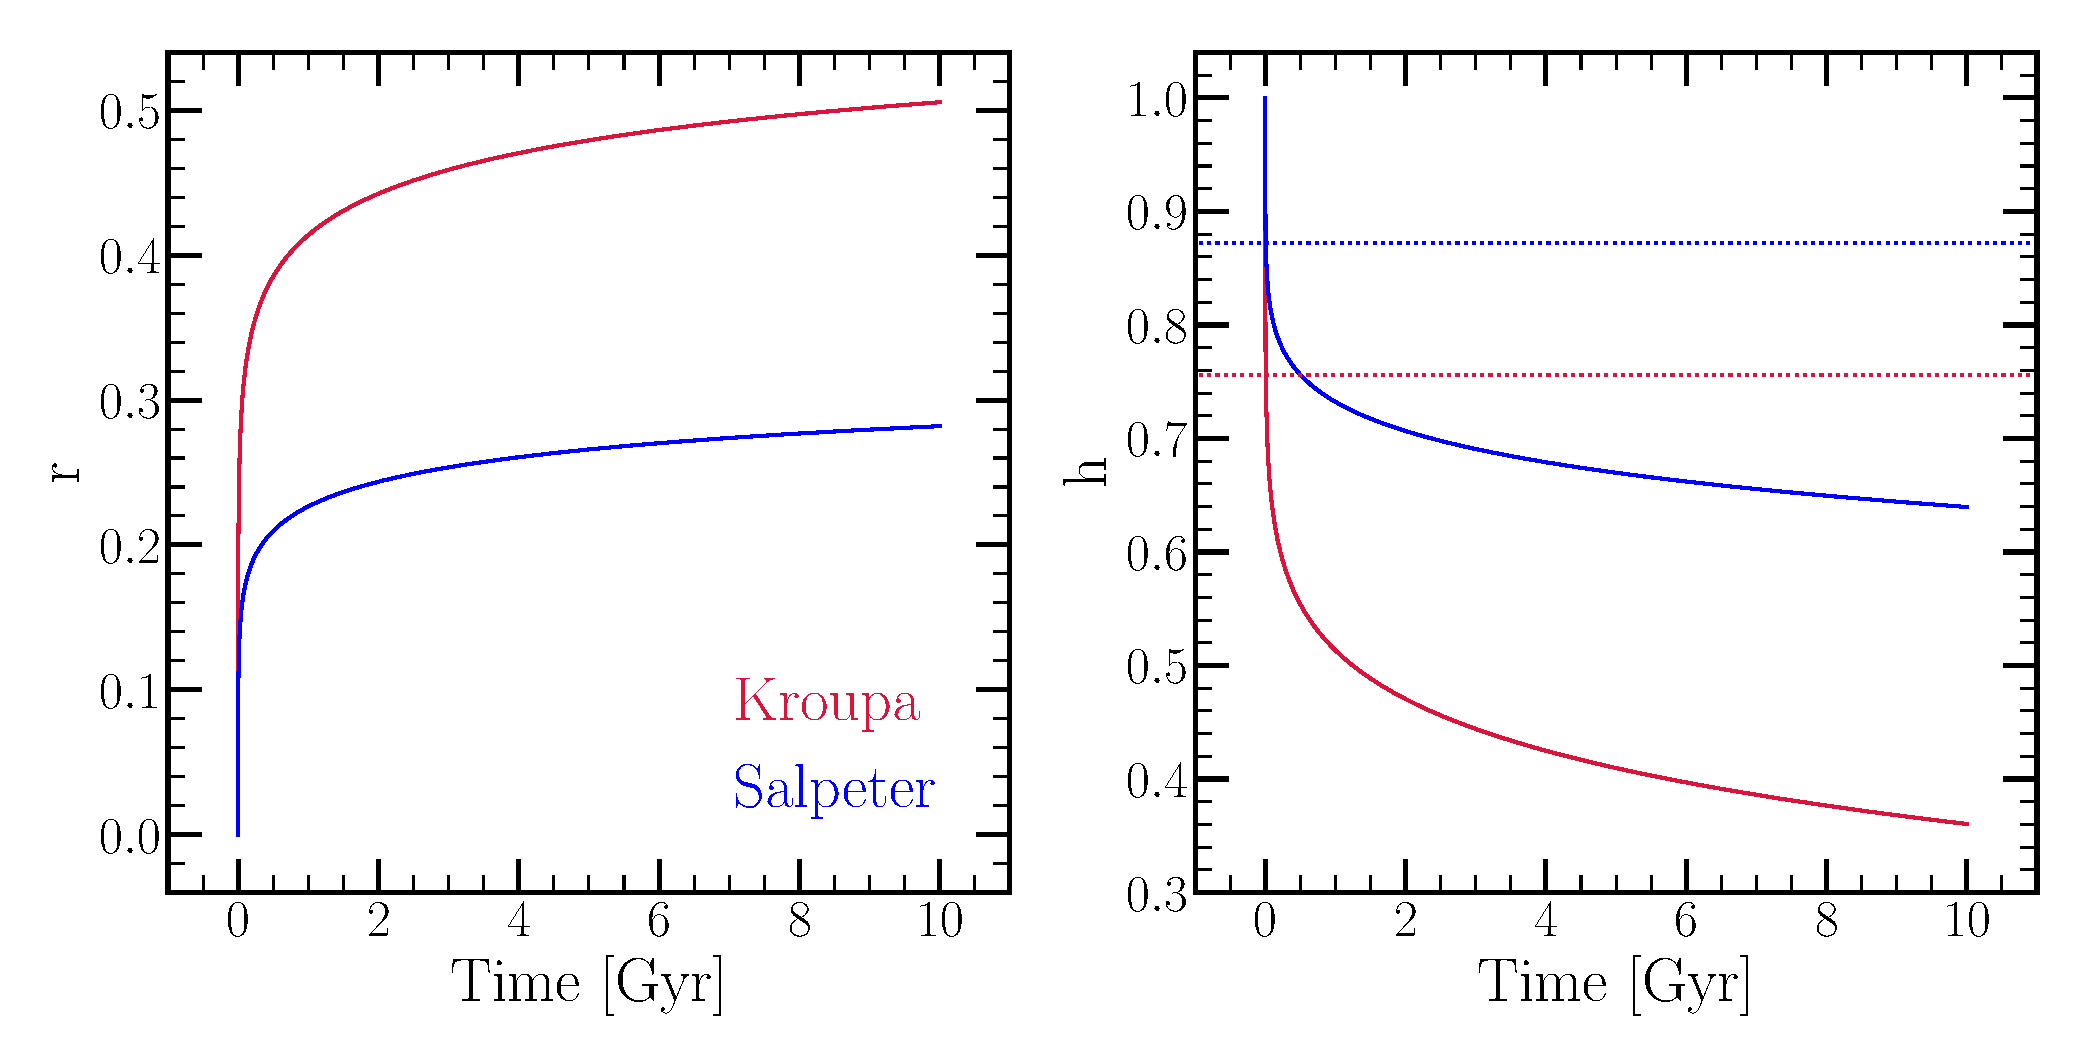
\includegraphics[scale = 0.47]{rh_2panel.pdf}
\caption{\textbf{Left}: The cumulative return fraction $r$ for a single 
stellar population as a function of time for both Kroupa (red) and Salpter 
(blue) initial mass functions~\citep{Kroupa2001,Salpeter1955}. } 
\label{fig:rh_2panel}
\end{figure*}

\null\par\noindent
\hypertarget{sec:enrichment}{\textbf{4) Enrichment}} \par\noindent 
In this section we present the equations detailing the time-dependent 
enrichment of a given element in the single-zone approximation and how they 
are implemented numerically in \texttt{VICE}. The time-derivative of the total 
mass of an element $x$ is given by: 
\begin{equation}
\dot{M}_\text{x} = \dot{M}_\text{x}^\text{CC} + \dot{M}_\text{x}^\text{Ia} + 
\dot{M}_\text{x}^\text{AGB} - \frac{M_\text{x}}{M_\text{g}}[\dot{M}_* + 
\xi_\text{enh}\dot{M}_\text{out}] + \dot{M}_\text{returned} + 
Z_\text{x,in}\dot{M}_\text{in}
\end{equation}
This equation is simply a mathematical statement of the source and sink terms 
of a given element in the ISM. At any given time, an arbitrary element will 
have a given emount of enrichment from core collapse supernovae 
[$\dot{M}_\text{x}^\text{CC}$], type Ia supernovae [$\dot{M}_\text{x}^\text{
Ia}$], and AGB stars [$\dot{M}_\text{x}^\text{AGB}$]. At the same time, it 
is depleted from the ISM as stars are formed at its metallicity 
[$(M_\text{x}/M_\text{g})\dot{M}_*$] and ejected in outflows at some 
multiplicative factor of the ISM metallicity [$(M_\text{x}/M_\text{g})
\dot{M}_\text{out}\xi_\text{enh}$]. It is also returned to the ISM as previous 
generations of stars evolve off the main sequence and return gas to the ISM 
at their birth metallicity [$\dot{M}_\text{returned}$]. If there is an 
inflow with nonzero metallicity, this also adds mass to the ISM 
[$Z_\text{x,in}\dot{M}_\text{in}$]. \texttt{VICE} implements the simplest 
approximation: 
\begin{equation}
\Delta M_\text{x} = \dot{M}_\text{x}^\text{CC}\Delta t + \dot{M}_\text{x}^\text{
Ia}\Delta t + \dot{M}_\text{x}^\text{AGB}\Delta t- \frac{M_\text{x}}
{M_\text{g}}[\dot{M}_* + \xi_\text{enh}\dot{M}_\text{out}]\Delta t + 
\Delta M_\text{returned} + Z_\text{x,in}(t)\dot{M}_\text{in}\Delta t
\end{equation}
The user has a large degree of customizability over every term on the 
right-hand side of this equation in \texttt{VICE}. We detail the treatment 
of each term individually. 
\par
In this section we do not detail the mathematical formalism of the 
nucleosynthetic yields from the various channels. We reserve this discussion 
for section~\hyperlink{sec:yields}{5}. 

\null\par\noindent
\hypertarget{sec:ccsne}{\textbf{4.1) Core Collapse Supernovae}} 
\par\noindent
Core collapse supernovae (CCSNe) are the thermonuclear detonations of massive 
stars ($\gtrsim8M_\odot$) at the end of their lifetimes. These stars live on 
extremely short timescales ($\sim$few Myr) compared to the relevant timescales 
for galaxy evolution ($\sim$few Gyr). Thus it is an excellent approximation to 
treat the CCSNe associated with an episode of star formation and their ensuing 
metal enrichment as instantaneous. This implies a direct linear relationship 
between the core-collapse production and the star formation rate: 
\begin{equation}
\label{eq:mdot_cc}
\dot{M}_\text{x}^\text{CC} = y_\text{x}^\text{CC}(Z)\dot{M}_*
\end{equation}
where $y_\text{x}^\text{CC}$ is the IMF-integrated core-collapse yield. This 
is the fraction of an entire stellar population's initial mass which is 
converted to an element $x$ at a metallicity $Z = M_\text{x}/M_\text{g}$. 
\begin{equation}
y_\text{x}^\text{CC}(Z) = \ddfrac{
	\int_8^u M_\text{x}\ddfrac{dN}{dM}dM
}{
	\int_l^u M\ddfrac{dN}{dM}dM
}
\end{equation}
where $M_\text{x}$ is the mass of element $x$ that is produced on average in 
the CCSN of a star with initial mass $M$. The bounds of the integral in the 
numerator are from 8 to $u$, because \texttt{VICE} operates under the 
assumption that only $>8\ M_\odot$ stars explode as CCSNe. The denominator is 
simply the total mass of stars in a single stellar population. 
\par
\texttt{VICE} allows the user to specify any functional form for 
$y_\text{x}^\text{CC}(Z)$. It achieves this by sampling their functional yield 
at every $10^{-5}$ interval steps in $Z$ between $Z$ = 0 and $Z$ = 0.5, 
interpolating on the finely sampled grid at each timestep. This spans the 
range of physically realistic values in $Z$. With the star formation rate  
defined as a function of time either by user specification or by the 
relations outlined in section~\hyperlink{sec:gas_supply}{3}, the solution to 
equation~\ref{eq:mdot_cc} is unique. Due to the approximation of instantaneous 
detonation of core-collapse supernovae, equation~\ref{eq:mdot_cc} is perhaps 
the simplest relation implemented in \texttt{VICE}. 

\null\par\noindent
\hypertarget{sec:sneia}{\textbf{4.2) Type Ia Supernovae}} \par\noindent 
Type Ia supernovae (SNe Ia) are the thermonuclear detonations of white dwarf 
stars when they reach the Chandrasekhar limit ($\sim1.4M_\odot$). White 
dwarves (WDs) associated with a given stellar population (or associated time 
step in \texttt{VICE}) are formed from low-mass stars, and thus take a minimum 
amount of time to form. It isn't until after a single stellar population forms 
WDs that SNe Ia will detonate, enriching the ISM with heavy elements. 
\par 
In order to model the time-dependent enrichment of an element $x$ by SNe Ia, 
we employ a \textit{delay-time distribution} (DTD) denoted by $R_\text{Ia}(t)$. 
This denotes the rate of SNe Ia associated with a single generation of stars 
at a time $t$ following its formation, and thus has units of yr$^{-1}$. 
Then, at any given timestep, the rate of enrichment of elements $x$ is given 
by the star formation history weighted by the DTD up to a fractional yield: 
\begin{equation}
\dot{M}_\text{x}^\text{Ia}(t) = y_\text{x}^\text{Ia}\langle\dot{M}_*(t)
\rangle_\text{Ia} = \ddfrac{\int_0^{t-t_\text{D}} \dot{M}_*(t')
R_\text{Ia}(t - t')dt'}{\int_{t_\text{D}}^\infty R_\text{Ia}(t')dt'}
\end{equation}
where $t_\text{D}$ is the minimum delay time for SNe Ia. \texttt{VICE} allows 
the user to specify any positive definite numerical value in Gyr for this 
parameter. It also allows the user to specify their own functional form for 
$R_\text{Ia}(t)$. It then automatically normalizes the DTD in the following 
manner: 
\begin{equation}\begin{split}
\label{eq:dtd_reduced}
R_\text{Ia,reduced}(t) &= \ddfrac{R_\text{Ia}(t)}{\int_0^\infty 
R_\text{Ia}(t')dt'} \\ 
&\rightarrow 
\begin{dcases}
0 & (0 < t < t_\text{D}) \\ 
\ddfrac{R_\text{Ia}(t)}{\sum_{i = t_\text{D}/\Delta t}^{\text{13.8 Gyr}/\Delta 
t} R_\text{Ia}(t)\Delta t} & (t_\text{D} \leq t \leq \text{13.8 Gyr}) \\ 
0 & (t \geq \text{13.8 Gyr})  
\end{dcases}
\end{split}\end{equation}
At the beginning of each integration, \texttt{VICE} normalizes the 
user-specified DTD according to equation~\ref{eq:dtd_reduced}. The user does 
not need to worry about normalizing their custom functional forms of 
$R_\text{Ia}$; that is done automatically. At all subsequent timesteps, the 
rate of enrichment from all previous stellar populations is simply the sum 
total from all previous timesteps: 
\begin{subequations}\begin{align}
\label{eq:mdot_ia}
\dot{M}_\text{x}^\text{Ia} &= y_\text{x}^\text{Ia}\int_0^t\dot{M}_*(t')
R_\text{Ia,reduced}(t - t')dt'
\\
&\rightarrow y_\text{x}^\text{Ia}\sum_{i = 0}^{t/\Delta t}\dot{M}_*(i\Delta t)
R_\text{Ia,reduced} (t - i\Delta t)\Delta t 
\end{align}\end{subequations}
The fact that $R_\text{Ia}(t) = 0$ for $t$ < $t_\text{D}$ is folded into the 
definition of $R_\text{Ia,reduced}$ implemented in \texttt{VICE}. 
Equation~\ref{eq:mdot_ia} is simply a mathematical statement that a given 
episode of star formation (i.e. timestep) enriches the ISM via SNe Ia some 
amount of time later according to the normalized rate of WD detonations at 
that time, and the total enrichment at a given time is simply the sum over all 
previous episodes of star formation. 

\null\par\noindent
\hypertarget{sec:agb}{\textbf{4.3) Asymptotic Giant Branch Stars}} 
\par\noindent
Asymptotic giant branch (AGB) stars are evolved stars which have concluded 
their hydrogen and helium fuel sources. They have a core composed of carbon 
and oxygen with a helium-burning shell surrounding the core. AGB stars undergo 
dredge-up episodes in which the heavier nucleosynthetic products produced in 
the core are drawn to the envelope. When the star forms a planetary nebula, 
these products are ejected to the interstellar medium. 
\par
Naively, one would expect that a delay-time distribution similar to the 
treatment of SNe Ia (section~\hyperlink{sec:sneia}{3}) would suffice. However, 
this approach would by nature adopt the assumption that every element is 
enriched via AGB stars with the same delay-time distribution. This is likely 
true for SNe Ia because the nucleosynthesis in a white dwarf detonation should 
be independent of the progenitor star. Asymptotic giant branch stars have 
yields which are functions of mass and metallicity, which suggests that 
different elements would have different delay-time distributions, which would 
also vary with metallicity. 
\par
While this approach would not face any immediately obvious faults, it is one 
with hardly any theoretical or observational constraints on the relevant 
parameters. Instead, to retain full generality, \texttt{VICE} adopts a 
different implementation. 
\par
Because stars of a given mass have a given lifetime, the lookback time to an 
episode of star formation specifies the mass of the AGB stars associated with 
that population that are currently enriching the ISM. Under the assumption 
that stars have instantaneous post main sequence lifetimes (accurate 
to~$\sim$5-10\%, sufficient for the single-zone approximation), 
equation~\ref{eq:tau_ms} specifies the mass of an AGB star at a given lookback 
time. The question that remains is thus: how many AGB stars from a given 
lookback time are enriching the ISM? 
\par
This is directly dependent on the star formation rate at that timestep. In 
addressing this question, we use a bit of mathematical slight of hand, and 
introduce a familiar quantity which we will refer to as the 
\textbf{hydrogen burning mass fraction} - the mass fraction of a single 
stellar population that is still on the main sequence some time following its 
formation. It has the following analytic form: 
\begin{equation}
h = \ddfrac{
	\int_l^{m_\text{to}(t)}m\frac{dN}{dm}dm
}{
	\int_l^u m\frac{dN}{dm}dm
}
\end{equation}
At first glance, it would appear that $h(t) = 1 - r(t)$. However, this is 
not true due to remnant masses. As we will show after further detail, the 
approximation $h(t) \approx 1 - r(t)$ barely fails for the single zone 
approximation for a Kroupa IMF. 
\par
Because $h(t)$ does not take into account remnant masses, it is necessarily 
$\leq 1 - r(t)$. Continuing by adopting an IMF of the general form 
$\beta m^{-\alpha}$ as in previous sections: 
\begin{equation}\begin{split}
h &= \ddfrac{
	\int_l^{m_\text{to}(t)}\beta m^{1 - \alpha}dm
}{
	\int_l^u \beta m^{1 - \alpha}dm
} \\ 
&= \ddfrac{
	\ddfrac{1}{2 - \alpha}m^{2 - \alpha}\Big|_l^{m_\text{to}}
}{
	\ddfrac{1}{2 - \alpha}m^{2 - \alpha}\Big|_l^u
} \\
&= \ddfrac{
	m_\text{to}(t)^{2 - \alpha} - l^{2 - \alpha}
}{
	u^{2 - \alpha} - l^{2 - \alpha}
}
\end{split}\end{equation}
The final equality is an attractive statement to make, but much more careful 
consideration must be taken for piece-wise IMFs like Kroupa. In that case, 
the second equality becomes: 
\begin{equation}\begin{split}
h = \ddfrac{
	\Big[\sum_i \ddfrac{1}{2 - \alpha_i}m^{2 - \alpha_i}\Big]_l^{m_\text{to}(t)}
}{
	\Big[\sum_i \ddfrac{1}{2 - \alpha_i}m^{2 - \alpha_i}\Big]_l^u
}
\end{split}\end{equation}
where the summation is over the relevant piece-wise mass ranges. In the case 
of the Kroupa IMF, $\alpha$ = 0.3 [1.3] [2.3] for stellar masses in the 
range $\leq0.08 M_\odot$ [$0.08 M_\odot\leq M \leq0.5 M_\odot$] 
[$\geq M_\odot$]. 
\par
With the star formation history $\dot{M}_*(t)$ and the yield as a function of 
turnoff mass and metallicity $Z$, $h$ constrains the time-derivative of the 
mass of a given element in the following manner: 
\begin{equation}\begin{split}
\dot{M}_\text{AGB} &= \int_0^t y(M_\text{to}(t'), Z_\text{ISM}(t')) 
\dot{M}_*(t') \dot{h}(t - t')dt \\ 
&\rightarrow \sum_{i = 0}^{t/\Delta t} y(M_\text{to}(i\Delta t), 
Z_\text{ISM}(i\Delta t)) \dot{M}_*(t - i\Delta t)[h(i\Delta t) - 
h((i + 1)\Delta t)] 
\end{split}\end{equation}
This numerical approximation may appear at first glance to have an artificial 
minus sign inserted into it when compared to equation~\ref{eq:crf_numerical},  
but this arises simply because $\dot{h}$ < 0. 
\par
In the right-hand panel of figure~\ref{fig:rh_2panel}, we show numerical 
calculations of $h$ against time in Gyr. At $t \approx$ 10 Gyr, $h \approx$ 
0.35 and $r \approx$ 0.5 for a Kroupa IMF. This suggests that adopting 
$1 - r(t)$ instead of $h(t)$ to describe the time-dependent enrichment from 
AGB stars from a single stellar population would systematically underpredict 
the enrichment of all elements produced in AGB stars. This is because it is a 
star's total initial mass which determines the net nucleosynthetic yield of a 
given element, and that includes the mass of the remnant that it will leave 
behind. 
\par



\null\par\noindent
\hypertarget{sec:yields}{\textbf{5) Nucleosynthetic Yields}} \par\noindent
In this section we detail the mathematical formulation of the nucleosynthetic 
yields implemented in \texttt{VICE}. 

\null\par\noindent
\hypertarget{sec:ccsne_yields}{\textbf{5.1) Core-Collapse Supernovae Yields}}
\par\noindent 
Enrichment from core-collapse supernovae (CCSNe) in \texttt{VICE} has an 
extremely simple analytic form, which arises from the assumption of 
instantaneous explosion (section~\hyperlink{sec:ccsne}{4.1}). The form of 
equation~\ref{eq:mdot_cc} dictates that $y_\text{x}^\text{CC}$ denote the 
fractional of a stellar population's mass that is converted into a given 
element $x$. For this reason, it is referred to as the \textit{IMF-integrated 
fractional yield}: 
\begin{equation}
y_\text{x}^\text{CC}(Z) = \ddfrac{
	\int_8^u m_\text{x}(m | Z)\frac{dN}{dm}dm
}{
	\int_l^u m\frac{dN}{dm}dm
}
\end{equation}
Under the well-founded assumption that only stars with initial masses 
$\geq 8 M_\odot$ explode as CCSNe, this equation is simply the mathematical 
statement that the fractional mass yield is simply the total mass produced by 
each individual CCSN divided by the total mass of the stellar population. 
\par
Here $m_\text{x}(m | Z)$ is the mass expelled into the ISM from a star with 
initial mass $m$ and metallicity $Z$. Unfortunately, this quantity is not 
well understood. In practice, it is determined for individual elements via 
tracer particles in numerical simulations~\citep{Woosley1995,Chieffi2004,
Chieffi2013,Limongi2018} on a grid of stellar masses and metallicities. 
The results are highly model-dependent, often assuming dialed-in explosion 
energy due to the computational expense involved in simulating supernovae. 
For this reason, \texttt{VICE} makes no assumptions about the user's 
preferred form of $y_\text{x}^\text{CC}(Z)$. It is left as a free parameter 
for the user to fully customize into an arbitrary function of metallicity 
$Z$ for each individual element. 

\null\par\noindent
\hypertarget{sec:sneia_yields}{\textbf{5.2) Type Ia Supernovae Yields}}
\par\noindent 
Enrichment via type Ia supernovae (SNe Ia), as discussed in 
section~\hyperlink{sec:sneia}{4.2}, is a delayed enrichment. A single stellar 
population's lower mass stars must first evolve off the main sequence and form 
white dwarves, which then explode at some rate $R_\text{Ia}(t)$. In keeping 
with the formulation of \textit{fractional} yields adopted in the treatment of 
CCSNe, $y_\text{x}^\text{Ia}$ denotes the fraction of a single stellar 
population's mass that is converted into an element $x$ over the full duty 
cycle of the delay-time distribution. Thus the only pieces of information 
required are the mass of an element $x$ produced in one instance of a 
SN Ia and the number of instances of SNe Ia can be expected for a given 
stellar population. 
\par
\citet{Maoz2012} found that $N_\text{Ia}/M_* = 2\pm1\times10^{-3} M_\odot^{-1}$, 
or that between 1 and 3 SNe Ia events can be expected per 1000 $M_\odot$ of 
star formation, with \citet{Andrews2017} and \citet{Weinberg2017} adopting 
$N_\text{Ia}/M_* = 2.2\times10^{-3} M_\odot^{-1}$ off of their best-fit 
parameters. This places a theoretical upper-bound on $y_\text{x}^\text{Ia}$ for 
any given element $x$. In the limit that every SN Ia is a collision between 
two near Chandrasekhar-mass WDs, the mass available for nuclear fusion 
is~$\sim2.8 M_\odot$. If all of this mass is converted into one element $x$, 
then $y_\text{x}^\text{Ia} = (2.8)(2.2\times10^{-3}) = 6.2\times10^{-3}$. 
\par
Similar to the yields from CCSNe, \texttt{VICE} allows users to customize 
their yields from SNe Ia, allowing any numerical value to be specified as 
$y_\text{x}^\text{Ia}$. There is little motivation for a metallicity-dependent 
yields from SNe Ia. It is possible that small amounts of iron-peak elements 
present in a WD may influence their nucleosynthetic yields; in this interest 
as well as for simple customizability, a future update to \texttt{VICE} will 
include functionality for $y_\text{x}^\text{Ia}$ to be a function of 
metallicity $Z$. 
\par


\null\par\noindent
\hypertarget{sec:tests}{\textbf{6) Tests}} \par\noindent 
In this section we present results quantifying \texttt{VICE}'s integration 
time as a function of the number of elements simulated and the timestep size. 
As detailed in previous sections, at each timestep, \texttt{VICE} determines 
the enrichment of all elements from all previous timesteps. As with any 
other time-step style integration, the amount of data to process and thus 
the integration time scale with the square of the number of timesteps 
(i.e. $T \propto (T_\text{end}/\Delta t)^2$). 
\par
Similarly, \texttt{VICE} treats every element independently. That is, the 
equations detailed in previous sections are not for any specific element - we 
purposefully did the analysis in full generality so that none of the 
simulation features in \texttt{VICE} needed to be changed to add new chemical 
elements. Since \texttt{VICE} conducts the same analysis for each element, 
we thus expect the integration time to scale linearly with the number of 
elements tracked per simulation (i.e. $T \propto N$). 
\par
Because \texttt{VICE} was implemented with the scientific motivation of 
studying the enrichment of oxygen, iron, and strontium, the first integrations 
were ran with these three elements, and with timesteps of $\Delta t$ = 1 Myr, 
each simulation finished in 20.4 seconds. With these proportionalities and 
this calibration, we expect the following scaling relation to describe the 
time per integration in \texttt{VICE} as a function of the number of 
elements $N$, end time $T_\text{end}$, and timestep $\Delta t$: 
\begin{equation}
T = \Big(\frac{\text{Processor Speed}}{2.7\text{ GHz}}\Big)^{-1}
N\Big(\frac{T_\text{end}/\Delta t}{10^4}\Big)^2(6.8\text{ seconds})
\end{equation}
Because 1 Myr is a relatively fine timestep, most integrations will typically 
not take this long. A more typical (and \texttt{VICE}'s default) timestep size 
would be expected to run in 68 milliseconds per element. 
\par
In figure~\ref{fig:timer} we present numerically calculated integration times 
for integrations over 5, 10, 15, 20, and 25 elements between $\Delta t$ = 
500 kyr and 10 Myr. We overplot as dotted lines in the corresponding color the 
expected $N\Delta t^{-2}$ fits for each line. We note first that for high 
$N$, this approximation underpredicts the integration time. Even though the 
mathematics is implemented uniformly for each element in \texttt{VICE}, there 
is still numerical overhead which increases with each element. For example, 
\texttt{VICE} will also take longer with more elements in determining the total 
metallicity at each timestep. Moreover, in writing output, \texttt{VICE} 
determines every [X/Y] abundance ratio - a calculation which scales with 
$N^2$. This is an effect which would be expected to mildly increase the 
sensitivity to the integration time for high $N$ simulations. In practice, we 
find that an $N^{1.1}$ scaling performs fine for most higher $N$ simulations. 


\begin{figure*} 
\centering
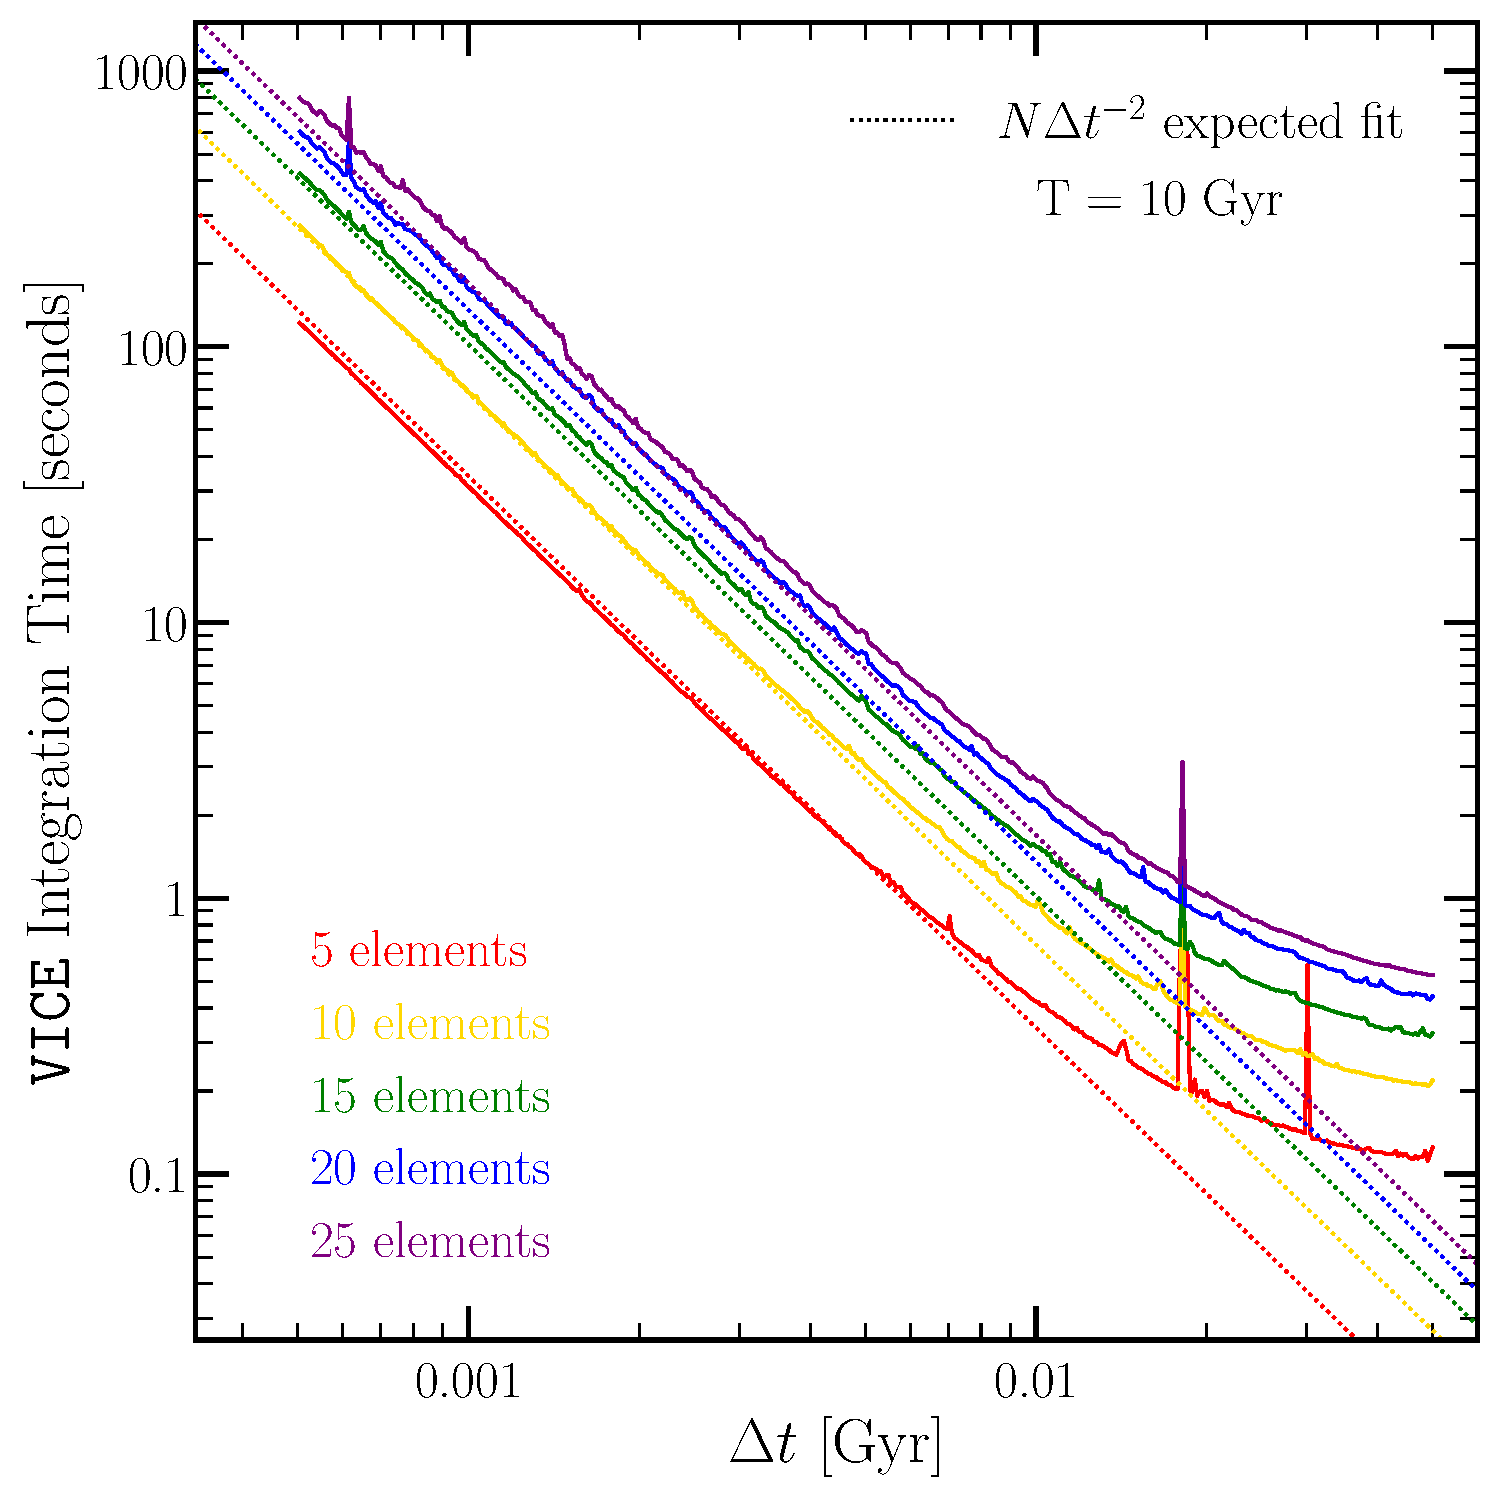
\includegraphics[scale = 0.4]{vice_timer.pdf}
\caption{Timed runs with $N$ = 5, 10, 15, 20, and 25 elements with timesteps 
ranging from 500 kyr to 10 Myr (solid lines) with an ending time of 
$T$ = 10 Gyr. We overplot the corresponding color-coded dotted lines showing 
the $N\Delta t^{-2}$ expected fit. The fit does well for low $N$, but 
mildly underpredicts the integration time for higher $N$. }
\label{fig:timer}
\end{figure*} 


\bibliographystyle{mnras}
\bibliography{science_documentation}

\end{document}

